%!TEX root = ../main.tex

% 1000-2000 words

\chapter{Design}

\section{Development Methodologies}

%TODO: Move to background study
\subsection{Waterfall}
The waterfall design methodology is a sequential design processed focused on the project progressing to each stage of development one at a time, for example, the design stage of the software would not take place until all requirements have been gathered and finalised.
Waterfall is considered to be a very structured methodology and is particularly useful when the requirements are well known and are fixed before the project begins and when the project and the technologies are well understood.

However, due to the rigidity of the Waterfall method, particularly around the planning phase, it is easy for mistakes made early on in the software development life cycle to become embedded within the project and be carried forward to later stages. CITATION NEEDED
For example, if a mistake is made during the requirements gathering phase and is not noticed until a later phase of the project, it will be very costly to change.

\subsection{Agile}
The Agile design methodology is a well established and iterative design process that involves regularly moving between the stages of the project in a non-sequential manner. 

One of the key principles of agile development is regular and iterative testing throughout the software development life cycle.
As I am a single developer working on this project, this is beneficial to me as it helps give early sight of potential design issues early in the project.

Agile is also very adaptable.
It allows for more flexibility to the software when design issues undoubtedly arise by not setting the specification for the whole project in stone too early.
By iteratively planning the design of the project, it allows for quick responses to feedback and if one part of the project is changed, it should have minimal effect on the rest of the project stages. 

The agile methodology also extends to the testing of the project.
By iteratively testing the software at various stages in the life cycle, it gives more chances to catch bugs early.
Under agile, defects discovered in software should be fixed as soon as possible after discovery \citep{beck2001agile}.

In a study by \cite{talby2006}, it was found that by following this practice, defects took less time to fix than without.
This may be due to the fact that the developed features are still fresh in the mind of the developer, and is therefore more easily able to see the problem area and fix.
The study also found that by keeping the bugs fixed and the code base stable throughout the project, it actually made the development phases of the project faster.
Furthermore, agile testing helps minimize the risks of bugs making it into the final artefact. 
If I were to have a single testing phase at the end of the project, it is possible that there would be more bugs than I had anticipated and that I would run out of time to properly fix them all. 
By using agile testing, this risk is minimized by allowing me to better manage the time of testing, as I will be able to delay or cancel the development of certain low priority features earlier in the project to allow me time to ensure a quality project.

\section{Development Processes}
There are also many sub-processes that are born out of or tie into Agile which could be beneficial for my project.

\subsection{Feature-Driven Development}
Feature-driven development (FDD) is an lightweight and iterative software development process which involves mapping out the feature list of the software as the `plan' for it's development.


\subsection{Test-Driven Development}
A key factor of test-driven development is planning out the testing phases of the project before the development of that phase begins.
The key workflow of TDD is as follows \citep{Beck:2002:TDD:579193}
\begin{enumerate}
	\item Add a test that tests the new feature works.
	\item Run all tests and see the new one fail.
	\item Write the code that makes the test pass.
	\item Run all tests and see them all succeed.
	\item Refactor the code and tests to remove duplication.
	\item Repeat.
\end{enumerate}

Under this process, a feature is complete when the tests show that it works.

A study by \cite{George:2003:IIT:952532.952753} developers following TDD produced higher quality code which passed 18\% more functional tests.

Furthermore, a software group at IBM made a drastic change to a TDD based workflow over their previously used ad-hoc testing approach and found that at the cost of a small drop in productivity, their defect rate was reduced by 50\%, the code quality was generally increased and was more flexible to changes and that morale was generally higher \citep{IBMTDD}. 
The paper also considered that the drop in productivity experienced may well have been down to the change to an unfamiliar system rather than an inherent flaw in TDD, but is not unusual that TDD would have this effect due to the increased time writing, preparing and running tests.
However, it must also be considered that if the practice offers a higher quality of code it is inherently likely to produce less errors and therefore the productivity/time trade-off may be worth it.
It is also noted that I must be prepared as I am unfamiliar with TDD myself, and will likely experience a similar drop in productivity as I begin to practice the methodology, however the paper offered several useful tips for developers/teams who are new to the practice.

\subsection{Behaviour-Driven Development}



After planning out the requirements, the next step in the design of KidQuest was to plan out the database structure.
I created an entity relationship to map out the various tables needed and the relationships between them.

\begin{figure}[t]
	\centering
	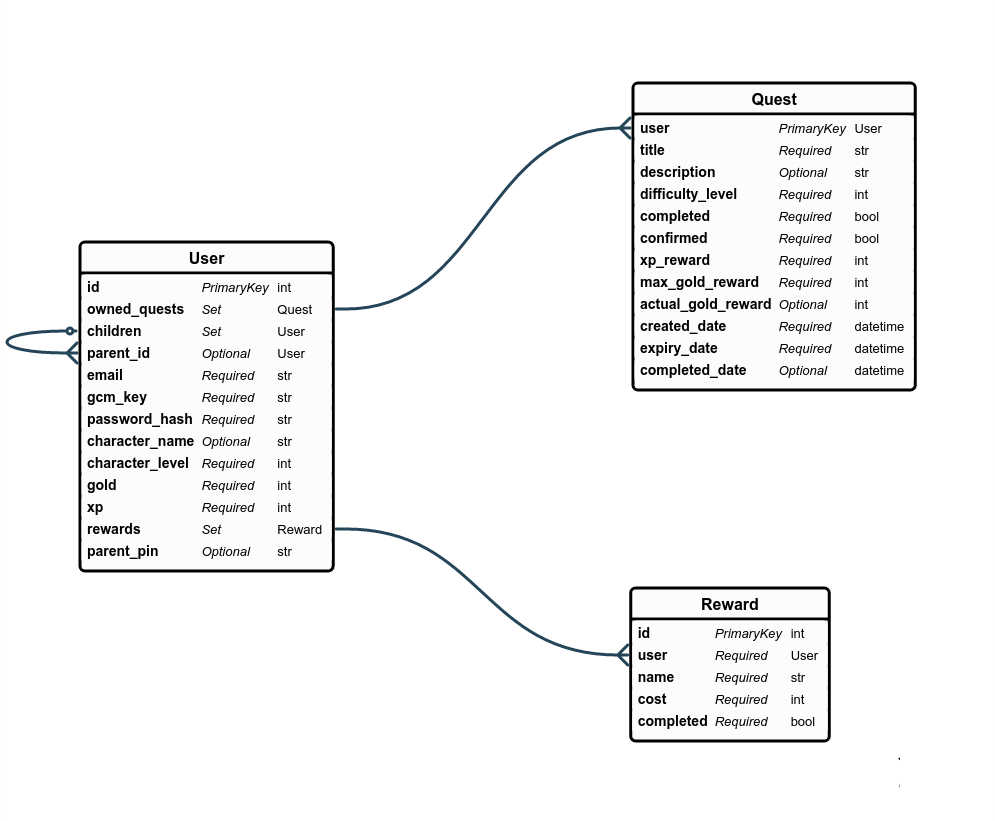
\includegraphics[width=0.75\textwidth]{images/entityRelationshipDiagram.png}
	\caption{Entity-Relationship Diagram}
	\label{fig:ERD}
\end{figure}

I have chosen to create the application in the Android SDK largely due to my previous experience with Java and Android. 
Furthermore, I believe Android is more applicable to the target audience of the app, as Android owns 82.8\% of the smartphone market share as of 2015.
%http://www.idc.com/prodserv/smartphone-os-market-share.jsp
I believe that parents are also more likely to buy their children Android phones than other brands due to the lower price point, making them more appealing when considering the likelihood of them being lost or broken by a child.

For the data analytics, I have opted to use web services written in Flask microframework for python, hosted on a server running Ubuntu Server 14.04. 
I have chosen python due to it's strong backing and community support in data analytics, and is one of the main languages of choice for scientists and statisticians.
The flask framework was chosen specifically as it is very simple to write and host RESTful APIs over the web.

To safely store and version control the code, I used a GitHub private repository to host my code in cloud storage. 
This allows me to better manage changes to the code-base. 

\section{Aesthetic Design}

\subsection{Wireframes}

\subsection{Android Developer Guidelines}
\section{Use Cases}	

\section{Development Style}

\section{Testing}

%TODO: Move these paragraphs to Design.
Unfortunately, when developing a REST API, it is difficult to manually write and send the request to the API to test it.
Programs and scripts exist to ease the process somewhat, but I found the easiest way to be automating the requests entirely. 
As a main principle of REST is to plan out the specific endpoints that can be messaged, it becomes rather simple to plan out tests in the form of sending an example of a valid and invalid request of each request type to each endpoint.
For example, the endpoint of `/api/users/<userId>/' allows two request types, GET and PUT, which generates four test cases.
\begin{itemize}
	\item{Valid GET}
	\item{Invalid GET}
	\item{Valid PUT}
	\item{Invalid put}
\end{itemize}  
%TODO: Research what test generation this is
However, this raises issues when considering that a request could be invalid for multiple reasons, and simply testing for invalid/valid may not reach adequate code coverage.
An example of this could be that a PUT request may be invalid due to an email address already existing within the database or because they have not included a valid did not include any new data about the user, which are two separate sections of the code that arguably each require their own tests.
Because of this, it must be analysed whether or not the test cases achieve sufficient code coverage, rather than just relying on the entry points into the software.
Luckily, the python package `coverage.py' allows for simple analysis of unit tests to determine the current code coverage for tests, which will provide a higher rate of confidence.

\subsection{Unit Testing} 
Unit Testing is integral to the workflow of test-driven development

\subsection{Integration Testing}
Integration testing encompasses tests that specifically test that the various parts of the project work together correctly.
For example, integration tests for KidQuest would test that the server and mobile app are able to correctly function together, by ensuring that the app can correctly send requests and that the server receives those requests as they were sent.


\subsection{Black Box Testing}

\subsection{White Box Testing}


\subsection{Regression Testing}
Regression testing is the practice of retesting the previously tested parts of the software to ensure that they are still performing correctly after a change elsewhere in the code, it can also be used to describe the process of testing previously detected and fixed bugs to determine that they have not reappeared.
This is made significantly easier by the implementation of strong automated unit tests, which allow me to quickly retest the majority of the code by rerunning the test suite.
I also intend to follow a common development practice where a unit test is added for each defect that is found within the code, a new unit test is added to detect the presence of that bug specifically. 
This will allow me to easily spot any recurrences of legacy bugs that would otherwise go unnoticed.